\documentclass{beamer}

\usetheme[progressbar=frametitle]{metropolis}
\usepackage{appendixnumberbeamer}
\usepackage{booktabs}
\usepackage{amsmath}
\usepackage{amssymb}
\usepackage{tcolorbox}
\usepackage{tikz}
\usepackage{multirow}
\usepackage{pdfpages}


\usetikzlibrary{automata, positioning, shapes}


\definecolor{metropolisblue}{RGB}{39, 59, 94}



% Begin document
\begin{document}

% Title page
\title{Sampling Methods}
\author{Nipun Batra}
\date{\today}
\institute{IIT Gandhinagar}
\maketitle

\begin{frame}{Topics}
    %TOC with enumerated items
    \setbeamertemplate{section in toc}[sections numbered]
    \tableofcontents

\end{frame}

\begin{frame}{Main Goal}
    \begin{itemize}
        \item We want to compute posterior predictive distribution (or something similar)
        \pause \item We would typically use Monte Carlo methods to do this.
        \pause \item $I = \int f(x) p(x) dx$ where $p(x)$ is the posterior distribution.
        \pause \item We can approximate $I$ by $\frac{1}{N} \sum_{i=1}^N f(x_i)$, where $x_i \sim p(x)$ are drawn \textbf{IID}.
        \pause \item Goal: sample from $p(x)$, usually using unnormalized density $\tilde{p}(x)$
    \end{itemize}
\end{frame}

\begin{frame}{Limitations of basic sampling methods}
    \begin{itemize}
        \item \textit{Transformation based methods}: Usually limited to drawing from standard distributions.
        \item \textit{Rejection and Importance sampling}: Require selection of good proposal distirbutions.
    \end{itemize}
    In high dimensions, usually most of the density $p(x)$ is concentrated within a tiny subspace of $x$. Moreover, those subspaces are difficult to be known a priori.

    A solution to these are Markov Chain Monte Carlo methods.
\end{frame}

\begin{section}{Markov Chains}

    %include 1-35 pages from hmm.pdf
    %\includepdf[pages=1-35]{hmm.pdf}


    \begin{frame}{Properties of Markov Chain: Stationarity}
        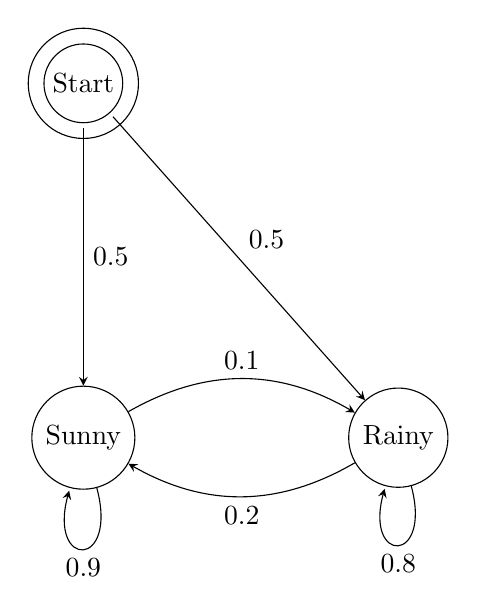
\begin{tikzpicture}[>=stealth, node distance=2cm, on grid, auto]
            \node[state, draw=none] (Start) {Start};
            \node[state, below=4.5cm of Start] (S) {Sunny};
            \node[state, right=4cm of S] (R) {Rainy};
            
            \path[->]
            (Start) edge node {0.5} (S)
            (Start) edge node {0.5} (R)
            (S) edge[loop below] node {0.9} (S)
            (S) edge[bend left] node {0.1} (R)
            (R) edge[loop below] node {0.8} (R)
            (R) edge[bend left] node {0.2} (S);
            
            % Adding concentric circles for the start state
            \draw (Start) circle (0.5);
            \draw (Start) circle (0.7);
        \end{tikzpicture}
  
    \end{frame}

    \begin{frame}{Properties of Markov Chain: Stationarity}

        Let us consider the rainy-sunny example.
      
        \begin{columns}[T] % Align columns at the top
          \begin{column}{0.48\textwidth} % First column
            \begin{table}[h]
              \centering
              \caption{Prior Probability (PI)}
              \begin{tabular}{cccc}
                \toprule
                & \(X_0 = \text{Sunny}\) & \(X_0 = \text{Rainy}\) \\
                \midrule
                PI & 0.5 & 0.5 \\
                \bottomrule
              \end{tabular}
            \end{table}
          \end{column}
          \begin{column}{0.48\textwidth} % Second column
            \begin{table}[h]
              \centering
              \caption{Transition Matrix (A)}
              \begin{tabular}{cccc}
                \toprule
                & & \multicolumn{2}{c}{\(X_{t+1}\)} \\
                \cmidrule{3-4}
                & & Sunny & Rainy \\
                \midrule
                \multirow{2}{*}{\(X_t\)} & Sunny & 0.9 & 0.1 \\
                & Rainy & 0.2 & 0.8 \\
                \bottomrule
              \end{tabular}
            \end{table}
          \end{column}
        \end{columns}

        \pause What is the probability of it being sunny on day 0?

    \pause 0.5
      \end{frame}

      \begin{frame}{Properties of Markov Chain: Stationarity}

        Let us consider the rainy-sunny example.
      
        \begin{columns}[T] % Align columns at the top
          \begin{column}{0.48\textwidth} % First column
            \begin{table}[h]
              \centering
              \caption{Prior Probability (PI)}
              \begin{tabular}{cccc}
                \toprule
                & \(X_0 = \text{Sunny}\) & \(X_0 = \text{Rainy}\) \\
                \midrule
                PI & 0.5 & 0.5 \\
                \bottomrule
              \end{tabular}
            \end{table}
          \end{column}
          \begin{column}{0.48\textwidth} % Second column
            \begin{table}[h]
              \centering
              \caption{Transition Matrix (A)}
              \begin{tabular}{cccc}
                \toprule
                & & \multicolumn{2}{c}{\(X_{t+1}\)} \\
                \cmidrule{3-4}
                & & Sunny & Rainy \\
                \midrule
                \multirow{2}{*}{\(X_t\)} & Sunny & 0.9 & 0.1 \\
                & Rainy & 0.2 & 0.8 \\
                \bottomrule
              \end{tabular}
            \end{table}
          \end{column}
        \end{columns}

        \begin{itemize}
            \item What is the probability of it being sunny on day 0?
            \pause \item 0.5

        \end{itemize}
      \end{frame}


      \begin{frame}{Properties of Markov Chain: Stationarity}

        Let us consider the rainy-sunny example.
      
        \begin{columns}[T] % Align columns at the top
          \begin{column}{0.48\textwidth} % First column
            \begin{table}[h]
              \centering
              \caption{Prior Probability (PI)}
              \begin{tabular}{cccc}
                \toprule
                & \(X_0 = \text{Sunny}\) & \(X_0 = \text{Rainy}\) \\
                \midrule
                PI & 0.5 & 0.5 \\
                \bottomrule
              \end{tabular}
            \end{table}
          \end{column}
          \begin{column}{0.48\textwidth} % Second column
            \begin{table}[h]
              \centering
              \caption{Transition Matrix (A)}
              \begin{tabular}{cccc}
                \toprule
                & & \multicolumn{2}{c}{\(X_{t+1}\)} \\
                \cmidrule{3-4}
                & & Sunny & Rainy \\
                \midrule
                \multirow{2}{*}{\(X_t\)} & Sunny & 0.9 & 0.1 \\
                & Rainy & 0.2 & 0.8 \\
                \bottomrule
              \end{tabular}
            \end{table}
          \end{column}
        \end{columns}

        \begin{itemize}
            \item What is the probability of it being sunny/rainy on day 1?
            \pause \item We can have two cases:
            \begin{itemize}
                \item $X_0 = \text{Sunny}$: $P(X_1 = \text{Sunny}) = 0.9$
                \item $X_0 = \text{Rainy}$: $P(X_1 = \text{Sunny}) = 0.2$   
                \item $P(X_1 = \text{Sunny}) = 0.5 \times 0.9 + 0.5 \times 0.2 = 0.55$
                \item $P(X_1 = \text{Rainy}) = 0.5 \times 0.1 + 0.5 \times 0.8 = 0.45$
            \end{itemize}
                

        \end{itemize}
      \end{frame}

      \begin{frame}{Properties of Markov Chain: Stationarity}

        Let us consider the rainy-sunny example.
      
        \begin{columns}[T] % Align columns at the top
          \begin{column}{0.48\textwidth} % First column
            \begin{table}[h]
              \centering
              \caption{Prior Probability (PI)}
              \begin{tabular}{cccc}
                \toprule
                & \(X_0 = \text{Sunny}\) & \(X_0 = \text{Rainy}\) \\
                \midrule
                PI & 0.5 & 0.5 \\
                \bottomrule
              \end{tabular}
            \end{table}
          \end{column}
          \begin{column}{0.48\textwidth} % Second column
            \begin{table}[h]
              \centering
              \caption{Transition Matrix (A)}
              \begin{tabular}{cccc}
                \toprule
                & & \multicolumn{2}{c}{\(X_{t+1}\)} \\
                \cmidrule{3-4}
                & & Sunny & Rainy \\
                \midrule
                \multirow{2}{*}{\(X_t\)} & Sunny & 0.9 & 0.1 \\
                & Rainy & 0.2 & 0.8 \\
                \bottomrule
              \end{tabular}
            \end{table}
          \end{column}
        \end{columns}

        \begin{itemize}
            \item What is the probability of it being sunny/rainy on day 2?
            \pause \item We can have two cases:
            \begin{itemize}
                \item $P(X_2 = \text{Sunny}) = 0.55 \times 0.9 + 0.45 \times 0.2 = 0.585$
                \item $P(X_2 = \text{Rainy}) = 0.55 \times 0.1 + 0.45 \times 0.8 = 0.415$
            \end{itemize}
                

        \end{itemize}
      \end{frame}

      \begin{frame}{Properties of Markov Chain: Stationarity}

        Let us consider the rainy-sunny example.
      
        \begin{columns}[T] % Align columns at the top
          \begin{column}{0.48\textwidth} % First column
            \begin{table}[h]
              \centering
              \caption{Prior Probability (PI)}
              \begin{tabular}{cccc}
                \toprule
                & \(X_0 = \text{Sunny}\) & \(X_0 = \text{Rainy}\) \\
                \midrule
                PI & 0.5 & 0.5 \\
                \bottomrule
              \end{tabular}
            \end{table}
          \end{column}
          \begin{column}{0.48\textwidth} % Second column
            \begin{table}[h]
              \centering
              \caption{Transition Matrix (A)}
              \begin{tabular}{cccc}
                \toprule
                & & \multicolumn{2}{c}{\(X_{t+1}\)} \\
                \cmidrule{3-4}
                & & Sunny & Rainy \\
                \midrule
                \multirow{2}{*}{\(X_t\)} & Sunny & 0.9 & 0.1 \\
                & Rainy & 0.2 & 0.8 \\
                \bottomrule
              \end{tabular}
            \end{table}
          \end{column}
        \end{columns}

        \begin{itemize}
            \item What is the probability of it being sunny/rainy on day $T$?
            \pause \item We can use matrix power to compute this.
            \pause \item Distribution of $X_T$ is given by $\pi = \pi POWER(A, T)$.
            \pause \item At $T=99$ and $T=100$, $\pi = (0.67, 0.33)$.

        \end{itemize}
      \end{frame}
      
    

    \begin{frame}{Properties of Markov Chain: Stationarity}
        Notebook: markov-chain.ipynb

        Questions:
        \begin{itemize}
            \item Does the distribution of $X_T$ depend on initial distribution $\pi$?
        \end{itemize}
        
    \end{frame}

    \begin{frame}{Properties of Markov Chain: Stationarity}
    We can define statationary distribution as follows:
    \begin{itemize}
        \item A distribution $\pi$ is said to be stationary for a Markov chain with transition matrix $A$ if $\pi = \pi A$.
        \item For previous example, 
        \begin{itemize}
            \item $\pi = (\pi_1, \pi_2)$
            \item $\pi_1 = 0.9 \pi_1 + 0.2 \pi_2$
            \item $\pi_2 = 0.1 \pi_1 + 0.8 \pi_2$
            \item $\pi_1 + \pi_2 = 1$
            \item Solving, $\pi = (\frac{2}{3}, \frac{1}{3})$
        \end{itemize}   
    \end{itemize}     
    \end{frame}

    \begin{frame}{Properties of Markov Chain: Stationarity}
        Can we have a Markov chain with multiple stationary distributions?
    
        \pause   \begin{columns}[T] % Align columns at the top
            \begin{column}{0.48\textwidth} % First column for TikZ diagram
              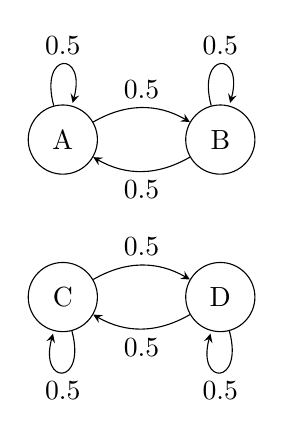
\begin{tikzpicture}[>=stealth, node distance=2cm, on grid, auto]
                \node[state] (A) {A};
                \node[state, right=2cm of A] (B) {B};
                \node[state, below=2cm of A] (C) {C};
                \node[state, right=2cm of C] (D) {D};
                
                \path[->]
                (A) edge[loop above] node {0.5} (A)
                (A) edge[bend left] node {0.5} (B)
                (B) edge[loop above] node {0.5} (B)
                (B) edge[bend left] node {0.5} (A)
                (C) edge[loop below] node {0.5} (C)
                (C) edge[bend left] node {0.5} (D)
                (D) edge[loop below] node {0.5} (D)
                (D) edge[bend left] node {0.5} (C);
              \end{tikzpicture}
            \end{column}
            \begin{column}{0.48\textwidth} % Second column for the table
              \begin{table}[h]
                \centering
                \caption{Transition Matrix (A)}
                \small 
                \begin{tabular}{cccccc}
                  \toprule
                  & & \multicolumn{4}{c}{\(X_{t+1}\)} \\
                  \cmidrule{3-6}
                  & & A & B & C & D \\
                  \midrule
                  \multirow{4}{*}{\(X_t\)} & A & 0.5 & 0.5 & 0 & 0 \\
                  & B & 0.5 & 0.5 & 0 & 0 \\
                  & C & 0 & 0 & 0.5 & 0.5 \\
                  & D & 0 & 0 & 0.5 & 0.5 \\
                  \bottomrule
                \end{tabular}
              \end{table}
            \end{column}
          \end{columns}

          \pause \begin{itemize}
            \item If we start at $A$ or $B$, the stationary distribution is $(0.5, 0.5, 0, 0)$.
            \item If we start at $C$ or $D$, the stationary distribution is $(0, 0, 0.5, 0.5)$.
          \end{itemize}

        \end{frame}

\end{section}

\begin{frame}{Properties of Markov Chain: Time Homogeneity}
    \begin{itemize}
        \item A Markov chain is said to be \textbf{homogeneous} if the transition probabilities are independent of the time $t$.
        \pause \item We have the same transition matrix $A$ for all $t$.
    \end{itemize}
    
\end{frame}


\begin{frame}{Properties of Markov Chain: Irreducibility}
    \begin{itemize}
        \item A Markov chain is said to be \textbf{irreducible} if every state is accessible from every other state.
        \pause \item In other words, there is a non-zero probability of reaching any state from any other state.
    \end{itemize}

    
\end{frame}
\begin{frame}{Properties of Markov Chain: Aperiodicity}
    \begin{itemize}
        \item A Markov chain is said to be \textbf{aperiodic} if the greatest common divisor of the set of all possible times between return to a state is 1.
        \pause \item In other words, the chain does not return to a state in a periodic fashion.
        \pause \item A simple check: can every state be reached in two consecutive timestamps?
        
    \end{itemize}

    \pause Example 1

    \begin{table}[h]
      \centering
      \caption{Transition Matrix (A)}
      \begin{tabular}{cccc}
        \toprule
        & & \multicolumn{2}{c}{\(X_{t+1}\)} \\
        \cmidrule{3-4}
        & & Sunny & Rainy \\
        \midrule
        \multirow{2}{*}{\(X_t\)} & Sunny & 0.9 & 0.1 \\
        & Rainy & 0.2 & 0.8 \\
        \bottomrule
      \end{tabular}
    \end{table}

    \pause Can we be in Rainy or Sunny state at $t=0$ and $t=1$. 

    \pause Yes -> Aperiodic

  \end{frame}

%  \begin{frame}{Properties of Markov Chain: Aperiodicity}
%    \begin{itemize}
%        \item A Markov chain is said to be \textbf{aperiodic} if the greatest common divisor of the set of all possible times between return to a state is 1.
%        \pause \item The chain does not return to a state in a periodic fashion.
%        \pause \item A simple check: can every state be reached in two consecutive timestamps?
%        
%    \end{itemize}
%  
%    \pause Example 1
%  
%    
%      \begin{tabular}{cccc}
%        \small
%        \toprule
%        & & \multicolumn{2}{c}{\(X_{t+1}\)} \\
%        \cmidrule{3-4}
%        & & Sunny & Rainy \\
%        \midrule
%        \multirow{2}{*}{\(X_t\)} & Sunny & 0.9 & 0.1 \\
%        & Rainy & 0.2 & 0.8 \\
%        \bottomrule
%      \end{tabular}
%  
%  
%    \pause Can we be in Rainy or Sunny state at $t=0$ and $t=1$. 
%  
%    \pause Yes -> Aperiodic
%  
%  
%  
%  
%  
%  
%  \end{frame}

  \begin{frame}{Properties of Markov Chain: Aperiodicity}
    \begin{itemize}
        \item A Markov chain is said to be \textbf{aperiodic} if the greatest common divisor of the set of all possible times between return to a state is 1.
        \pause \item In other words, the chain does not return to a state in a periodic fashion.
        \pause \item A simple check: can every state be reached in two consecutive timestamps?
        
    \end{itemize}

    \pause Example 2

    \begin{table}[h]
      \centering
      \caption{Transition Matrix (A) for Four States}
      \small % Add \small to make the font size smaller
      \begin{tabular}{cccccc}
        \toprule
        & & \multicolumn{4}{c}{\(X_{t+1}\)} \\
        \cmidrule{3-6}
        & & State 1 & State 2 & State 3 & State 4 \\
        \midrule
        \multirow{4}{*}{\(X_t\)} & State 1 & 0 & 1 & 0 & 0 \\
        & State 2 & 0.5 & 0 & 0.5 & 0 \\
        & State 3 & 0 & 0.5 & 0 & 0.5 \\
        & State 4 & 0 & 0 & 1 & 0 \\
        \bottomrule
      \end{tabular}
    \end{table}

  
\end{frame}




\begin{frame}

\end{frame}

\begin{frame}{Irreducible Markov Chain (2 States)}
    \begin{columns}[T] % Align columns at the top
      \begin{column}{0.48\textwidth} % First column for irreducible Markov chain
        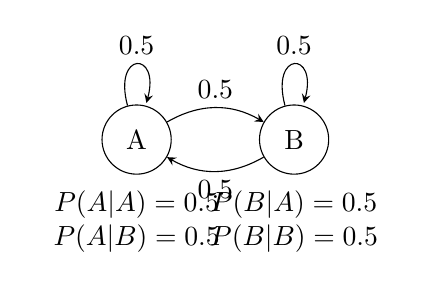
\begin{tikzpicture}[>=stealth, node distance=2cm, on grid, auto]
          \node[state] (A) {A};
          \node[state, right=2cm of A] (B) {B};
          
          \path[->]
          (A) edge[loop above] node {0.5} (A)
          (A) edge[bend left] node {0.5} (B)
          (B) edge[loop above] node {0.5} (B)
          (B) edge[bend left] node {0.5} (A);
          
          % Fill the transition matrix entries
          \node[below=0.5cm] at (A) {
            \begin{tabular}{c}
              $P(A|A) = 0.5$ \\
              $P(A|B) = 0.5$
            \end{tabular}
          };
          \node[below=0.5cm] at (B) {
            \begin{tabular}{c}
              $P(B|A) = 0.5$ \\
              $P(B|B) = 0.5$
            \end{tabular}
          };
        \end{tikzpicture}
      \end{column}
      \begin{column}{0.48\textwidth} % Second column for non-irreducible Markov chain
        % Add non-irreducible Markov chain TikZ code here
      \end{column}
    \end{columns}
  \end{frame}
  
  \begin{frame}{Non-Irreducible Markov Chain (2 States)}
    \begin{columns}[T] % Align columns at the top
      \begin{column}{0.48\textwidth} % First column for irreducible Markov chain
        % Add irreducible Markov chain TikZ code here
      \end{column}
      \begin{column}{0.48\textwidth} % Second column for non-irreducible Markov chain
        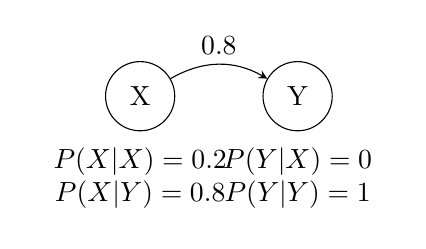
\begin{tikzpicture}[>=stealth, node distance=2cm, on grid, auto]
          \node[state] (X) {X};
          \node[state, right=2cm of X] (Y) {Y};
          
          \path[->]
          (X) edge[bend left] node {0.8} (Y);
          
          % Fill the transition matrix entries
          \node[below=0.5cm] at (X) {
            \begin{tabular}{c}
              $P(X|X) = 0.2$ \\
              $P(X|Y) = 0.8$
            \end{tabular}
          };
          \node[below=0.5cm] at (Y) {
            \begin{tabular}{c}
              $P(Y|X) = 0$ \\
              $P(Y|Y) = 1$
            \end{tabular}
          };
        \end{tikzpicture}
      \end{column}
    \end{columns}
  \end{frame}
  

\begin{section}{Markov Chain Monte Carlo (MCMC)}

    \begin{frame}{MCMC main idea}
        \begin{itemize}
            \item We identify a way to construct a `nice' Markov chain such that its stationary probability distribution $\pi(x)$ is our target distribution $p(x)$.
            \item We then run the Markov chain for a long time and use the samples to estimate $I$.
            \item But, we thus far said: $x_i \sim p(x)$ are drawn \textbf{IID}. 
            \item But, if we use a Markov chain to generate samples, then the samples are not i.i.d.
            \item But, we can still use the samples to estimate $I$ using the \textbf{ergodic theorem}.
            \item An irreducible, aperiodic, and stationary Markov chain has a unique stationary distribution $\pi$ and we can generate samples from $\pi$ and compute $I$.
        \end{itemize}
    \end{frame}
    


    \begin{frame}{Ergodic Theorem for Markov Chains}
        Inspired from: MathematicalMonk's playlisty on MCMC.

        \begin{itemize}
            \item From Monte Carlo sampling, we know we can estimate $I = \int f(x) p(x) dx$ by $\frac{1}{N} \sum_{i=1}^N f(x_i)$, where $x_i \sim p(x)$.
            \item But, the samples are drawn i.i.d. from $p(x)$.
            \item But, if we use a Markov chain to generate samples, then the samples are not i.i.d.
            \item But, we can still use the samples to estimate $I$ using the \textbf{ergodic theorem}.
        \end{itemize}
    \end{frame}


    \begin{frame}{Metropolis Hastings}
        \begin{itemize}
            \item The basic idea is propose to move to a new state $x_{i+1}$ from the current state $x_i$ with probability $q(x_{i+1}|x_i)$, where $q$ is called the proposal distribution and our target density of interest is $p (= \frac{1}{Z} \tilde{p})$.
            \item The new state is accepted with probability $\alpha(x_i, x_{i+1})$.
            \begin{itemize}
                \item If $p(x_{i+1}| x_i) = p(x_i| x_{i+1})$, then $\alpha(x_i, x_{i+1}) = \min (1, \frac{p(x_{i+1})}{p(x_i)})$.
                \item If $p(x_{i+1}| x_i) \neq p(x_i| x_{i+1})$, then $\alpha(x_i, x_{i+1}) = \min (1, \frac{p(x_{i+1})q(x_i|x_{i+1})}{p(x_i)q(x_{i+1}|x_i)}) = \min (1, \frac{\tilde{p}(x_{i+1})q(x_i|x_{i+1})}{\tilde{p}(x_i)q(x_{i+1}|x_i)})$
            \end{itemize}
            \item Evaluating $\alpha$, we only need to know the target distribution up to a constant of proportionality or without normalization constant.
        \end{itemize}
    \end{frame}

    \begin{frame}{Algorithm: Metropolis Hastings}
        \begin{enumerate}
            \item Initialize $x_0$.
            \item for $i = 1, \ldots, N$ do:
            \item \quad Sample $x^* \sim q(x^*|x_{i-1})$.
            \item \quad Compute $\alpha = \min (1, \frac{\tilde{p}(x^*)q(x_{i-1}|x^*)}{\tilde{p}(x_{i-1})q(x^*|x_{i-1})})$
            \item \quad Sample $u \sim \mathcal{U}(0, 1)$
            \item \quad if $u \leq \alpha$:
            
            \quad \quad $x_i = x^*$
            
            \quad else:
            
            \quad \quad $x_i = x_{i-1}$
        \end{enumerate}
    \end{frame}

    \begin{frame}{Pop Quiz}
        How do we choose the initial state $x_0$?
        \pause
        \begin{enumerate}
            \item Start the Markov Chain at an initial $x_0$.
            \item Using the proposal $q(x|x_i)$, run the chain long enough, say $N_1$ steps.
            \item Discard the first $N_1 - 1$ samples (called 'burn-in' samples).
            \item Treat $x_{N_1}$ as first sample from $p(x)$.
        \end{enumerate}
    \end{frame}

    \begin{frame}{MCMC demo}
        
        \url{https://chi-feng.github.io/mcmc-demo/app.html}
    \end{frame}
\end{section}

\end{document}